\documentclass[11pt,a4paper]{amsart}
\usepackage[utf8]{inputenc}
\usepackage[T1]{fontenc}
\usepackage{lmodern}
\usepackage{amsmath,amssymb,amsthm}
\usepackage{booktabs}
\usepackage{graphicx}
\graphicspath{{figures/}}
\usepackage{xcolor}
\usepackage[margin=2.5cm]{geometry}
\usepackage[colorlinks=true,linkcolor=blue!50!black,citecolor=blue!50!black,urlcolor=blue!50!black]{hyperref}

\newtheorem{theorem}{Theorem}[section]
\newtheorem{proposition}[theorem]{Proposition}
\newtheorem{lemma}[theorem]{Lemma}
\theoremstyle{remark}
\newtheorem{remark}[theorem]{Remark}
\numberwithin{equation}{section}
\emergencystretch=1.5em

\newcommand{\eg}{e^{\gamma}}
\newcommand{\sw}{\mathrm{sw}}

\title[Vector-sieve estimates for $p=m^2+n^2+1$]{An audit and restoration of the vector-sieve estimates for primes
of the form $m^2+n^2+1$ with $p+2$ almost prime}
\thanks{Code and data: \url{https://github.com/Ruqing1963/nath-xie-sieve-audit}}
\author{Ruqing Chen}
\address{GUT Geoservice Inc., Montreal, Canada}
\email{ruqing@hotmail.com}
\date{November 2026}
\subjclass[2020]{Primary 11N36; Secondary 11N05, 11N32}
\keywords{vector sieve, semi-linear sieve, linear sieve, Richert weights, primes $m^2+n^2+1$, almost primes}

\begin{document}

\begin{abstract}
Nath and Xie state that there are $\gg x(\log x)^{-5/2}$ primes $p\le x$ with $p=m^2+n^2+1$ and $\Omega(p+2)\le9$.
The proof combines a semi-linear and a linear sieve in a vector sieve, Iwaniec's switching principle and Richert's
weights, and ends with a numerical inequality $H>0$. We recompute that inequality. The linear sieve functions used in
the computation solve the delay system without the factor $1/s$, so that the computed lower function exceeds the
computed upper function; with the correct functions the quantities reported as $G=0.001378$ and $H=1.2690$ become
$-23.7$ and $-34.3$. We reproduce the reported values from the authors' code to three digits, which identifies the
cause. We also correct three constants in the switched term (one of them in the unsafe direction) and observe that the
levels in the switching step can be chosen more freely. With these changes the method of the paper gives
$\Omega(p+2)\le17$; with the constants as printed it gives $\Omega(p+2)\le59$.
\end{abstract}

\maketitle

\section{Introduction}\label{sec:intro}

Let $\Omega(n)$ be the number of prime factors of $n$ counted with multiplicity. Nath and Xie \cite{NX} state
\begin{equation}\label{eq:NXclaim}
\#\{p\le x:\ p=m^2+n^2+1,\ \Omega(p+2)\le 9\}\gg\frac{x}{(\log x)^{5/2}}
\end{equation}
\cite[Theorem~1.1]{NX}. The analytic part of the argument, Propositions~3.10 and~4.1--4.3 of \cite{NX}, reduces
\eqref{eq:NXclaim} to the positivity of an explicit function $H(\lambda,\theta,\theta_1,\theta_2)$ built from the
half-dimensional sieve functions $(F_1,f_1)$, the linear sieve functions $(F_2,f_2)$ and some Euler products, and
\cite[\S5]{NX} reports
\[
G(0.4230,0.0249)\approx0.001378,\quad H(0.17,0.25,0.449,0.011)=1.2690,\quad \tfrac1{0.17}+\tfrac1{0.25}=9.8824 .
\]
The function $G$ is $H$ without the weighted term, and it would give $\Omega(p+2)\le40$. The computations were
done with Matlab files that accompany the arXiv source of \cite{NX}. Section, equation and proposition numbers of
\cite{NX} refer to the arXiv version~3, which is the final version published in Acta Arithmetica. In this note we recompute $G$ and $H$ and the
constants that enter them, and we determine what the method gives once the computation is repaired. All numbers below
are produced by one script in the Python standard library, \texttt{code/verify\_nath\_xie.py}, which runs in about
15 seconds.

\begin{theorem}\label{thm:A}
\begin{enumerate}
\item The linear sieve functions in \cite[\S5]{NX} and in the accompanying code solve $F_2'=f_2(s-1)-F_2$,
$f_2'=F_2(s-1)-f_2$ instead of $(sF_2)'=f_2(s-1)$, $(sf_2)'=F_2(s-1)$. The computed $f_2$ exceeds the computed $F_2$
on $2.49<s<14.8$.
\item With the correct functions, $G(0.4230,0.0249)=-23.73$ and $H(0.17,0.25,0.449,0.011)=-34.28$, with the
constants as printed. The vector-sieve lower bound $f(\sigma_1,\sigma_2)$ is negative at the first point.
\item With the code's functions and constants we obtain $G(0.4230,0.0249)=-0.0009$, with largest admissible
$\theta_2$ equal to $0.0248$ instead of $0.0249$, and $H(0.17,0.25,0.449,0.011)=1.2625$. These agree with the reported
values once the two artefacts of the code are reproduced: the delay system above, and an optimiser that is
called on an empty constraint set.
\end{enumerate}
\end{theorem}

The half-dimensional functions are printed and coded correctly; in particular there is no factor $2$ missing in
$f_1$ (Section~\ref{sec:functions}). Theorem~\ref{thm:A} invalidates the numerical step of \cite{NX}, not the
propositions that precede it. We therefore ask what those propositions give with the correct functions.

\begin{theorem}\label{thm:B}
Assume Propositions~$3.10$, $4.1$ and $4.3$ of \cite{NX}, and replace Proposition~$4.2$ by
Proposition~\ref{prop:switch} below. Then
\[
\#\{p\le x:\ p=m^2+n^2+1,\ \Omega(p+2)\le 17\}\gg\frac{x}{(\log x)^{5/2}} .
\]
With Proposition~$4.2$ as printed, the same computation gives $\Omega(p+2)\le59$. Without Richert's weights it gives
$\Omega(p+2)\le48$, respectively $\le342$.
\end{theorem}

Proposition~\ref{prop:switch} differs from \cite[Proposition~4.2]{NX} in three respects
(Section~\ref{sec:constants}). (i)~In \cite{NX} the Wirsing constant $c_3$ lacks the Euler factor $(1-\frac12)^{1/2}$ of the
prime $2$. (ii)~The joint singular series of the two linear sieves is $\prod(1-(p-2)^{-2})$ rather than
$\prod(1+(p-2)^{-2})$. Moreover, the bound $H_1(m)\le\frac{2m}{\varphi(2m)}c_2$ is reversed; this is the one error
in the unsafe direction. (iii)~The levels $D_1\le x^{\theta_1}$ and $D_2\le x^{\theta_2}$ need not be capped
individually, since only $D_1D_2\le x^{1/2-\epsilon}$ is used. Items (i) and (ii) together halve the switched term,
and (iii) lowers it further at small $\theta_2$. The numerical values in Theorem~\ref{thm:B} come from a grid
search in floating point, not from interval arithmetic. The margin is $17.43<18$ for the bound $17$ and $59.20<60$
for the bound $59$. Replacing the rectangle bounds of the vector sieve by the Buchstab fixed point of
\cite{ChenXIV} lowers the bound further, to $\Omega(p+2)\le15$ (Remark~\ref{rem:buchstab}); this is not needed for
Theorem~\ref{thm:B}.

\section{The criterion}\label{sec:criterion}

We use the notation of \cite{NX}. Let $\gamma$ be Euler's constant, let $0<\theta_2<\theta_1<\frac12$ with
$\theta_1>\frac14$, and let $\theta_2<\theta<1$ and $\lambda>0$. The set $\mathcal A=\{p-1:\ p\le x-2,\ p\equiv3\
(8),\ (p+2,P(x^{\theta_2}))=1\}$ is sifted by the primes $q\equiv3\ (4)$ up to $x^{\theta_1}$. This is a sieve of
dimension $\kappa_1=\frac12$ with $\beta_1=1$. The shifted primes $p+2$ are sifted by all primes up to
$x^{\theta_2}$, a sieve of dimension $\kappa_2=1$ with $\beta_2=2$. The vector sieve of \cite[Proposition~3.10]{NX}, modelled on \cite[\S3.3]{HBL}, is applied at level
$x^{1/2-2\epsilon}$. With $\sigma_i=1/(2\theta_i)$, the lower and upper vector-sieve functions are
\cite[(3.13), (3.14), (5.1)]{NX}
\begin{align}
f(\sigma_1,\sigma_2)&=\sup\Bigl\{f_1(s_1)F_2(s_2)+F_1(s_1)f_2(s_2)-F_1(s_1)F_2(s_2):\
\tfrac{s_1}{\sigma_1}+\tfrac{s_2}{\sigma_2}=1,\ s_1\ge1,\ s_2\ge2\Bigr\},\label{eq:f}\\
F(\sigma_1,\sigma_2)&=\inf\Bigl\{F_1(s_1)F_2(s_2):\ \tfrac{s_1}{\sigma_1}+\tfrac{s_2}{\sigma_2}=1,\ s_1>0,\
s_2\ge1\Bigr\}.\label{eq:F}
\end{align}
Thus $f$ is a supremum over the splittings $D=D_1D_2$ of the level and $F$ is an infimum. Both are correct as
printed. The criterion of \cite[\S5]{NX} is
\begin{equation}\label{eq:H}
H(\lambda,\theta,\theta_1,\theta_2)=\frac{A\,f(\sigma_1,\sigma_2)}{\theta_1^{1/2}\theta_2}
-\frac{2c_1c_2^2c_3\,C(\theta_1)}{\theta_2\min(\theta_1,\frac12-\theta_2)}
-\lambda\frac{A\,I(\theta,\theta_1,\theta_2)}{\theta_1^{1/2}\theta_2}>0,
\end{equation}
which gives $\omega(p+2)<1/\lambda+1/\theta$. Here $A=C\kappa e^{-3\gamma/2}/4$, and
\begin{equation}\label{eq:CI}
C(\theta_1)=\int_0^{1-2\theta_1}\log\frac{1-\beta-\theta_1}{\theta_1}\,\frac{d\beta}{\beta^{1/2}(1-\beta)},\qquad
I(\theta,\theta_1,\theta_2)=\int_{\theta_2}^{\theta}\Bigl(1-\frac\alpha\theta\Bigr)
F\Bigl(\frac{1-2\alpha}{2\theta_1},\frac{1-2\alpha}{2\theta_2}\Bigr)\frac{d\alpha}\alpha .
\end{equation}
The function $G(\theta_1,\theta_2)$ is the sum of the first two terms of \eqref{eq:H}, and $G>0$ gives
$\omega(p+2)<1/\theta_2$. The three terms are the lower bound for $S(\mathcal A,\mathcal Q,x^{\theta_1})$
(Proposition~4.1), the switched upper bound for the Buchstab sum over $x^{\theta_1}<p_1\le x^{1/2}$
(Proposition~4.2, Iwaniec's switching \cite{Iw72}), and Richert's weighted sum (Proposition~4.3), all in units of $x(\log x)^{-5/2}$. The constants
are
\begin{align*}
C&=\tfrac94\prod_{p\equiv3(4),\,p>3}\Bigl(1-\frac{3p-1}{(p-1)^3}\Bigr)\prod_{p\equiv1(4)}\Bigl(1-\frac1{(p-1)^2}\Bigr)
=1.772720,\\
\kappa&=\Bigl(\frac\pi2\prod_{p\equiv3(4)}(1-p^{-2})\Bigr)^{1/2}=1.159643,\\
c_1&=\prod_{p>3}\Bigl(1+\frac1{(p-2)^2}\Bigr)=1.202503,\\
c_2&=\prod_{p>2}\Bigl(1-\frac1{(p-1)^2}\Bigr)=0.660162,
\end{align*}
together with $c_3$ (Section~\ref{sec:constants}). We have checked the Euler factors of $C$ against (4.5) of
\cite{NX}. The factor $(1-(p-2)^{-2})$ printed in Proposition~4.3 is a misprint for $(1-(p-1)^{-2})$. With it, $C$
would be $1.677294$; Section~5 of \cite{NX} and the code both use the correct value.

\section{The sieve functions}\label{sec:functions}

\subsection{Half-dimensional sieve}
By \cite[(14.2)--(14.3)]{FI}, $F_1(s)=2(\eg/\pi s)^{1/2}$ for $0<s\le2$ and
$f_1(s)=(\eg/\pi s)^{1/2}\int_1^s dt/\sqrt{t(t-1)}$ for $1\le s\le3$. The integral equals
$2\log(\sqrt s+\sqrt{s-1})=\log\bigl(1+2(s-1)+2\sqrt{s(s-1)}\bigr)$, which is the expression printed in \cite[\S5]{NX}.
So $f_1/F_1=\log(\sqrt s+\sqrt{s-1})$ on $[1,2]$; for example the ratio is $0.414667$ at $s=1/(2\cdot0.4230)$.
For larger $s$ the functions solve $F_1'=(f_1(s-1)-F_1)/(2s)$ and $f_1'=(F_1(s-1)-f_1)/(2s)$, which is the form
$(s^{1/2}F_1)'=\frac12s^{-1/2}f_1(s-1)$ of \cite[Lemma~3.6]{NX}. The printed system, the code and our recomputation
agree.

\subsection{Linear sieve}
The linear sieve functions satisfy $F_2(s)=2\eg/s$ for $0<s\le3$ and $f_2(s)=2\eg\log(s-1)/s$ for $2\le s\le4$, and
\begin{equation}\label{eq:lin}
(sF_2(s))'=f_2(s-1)\quad(s>3),\qquad (sf_2(s))'=F_2(s-1)\quad(s>2)
\end{equation}
\cite[(12.1)--(12.2)]{FI}; this is again \cite[Lemma~3.6]{NX} with $\kappa=1$. Section~5 of \cite{NX} instead
prints
\begin{equation}\label{eq:printed}
F_2'(s)=f_2(s-1)-F_2(s)\quad(s>3),\qquad f_2'(s)=F_2(s-1)-f_2(s)\quad(s>2),
\end{equation}
which drops the factor $1/s$ on the right. The code (\texttt{solve\_DDE\_2} in \texttt{lower\_f\_sigma.m} and
\texttt{upper\_F\_sigma.m}) integrates \eqref{eq:printed} from $s=2$ with the history $F_2=2\eg/s$, $f_2=0$ on
$[1,2]$. It therefore also discards the initial segment of $F_2$ on $[2,3]$ and that of $f_2$ on $[2,4]$. On
$[2,3]$, where $f_2(s-1)=0$, the code's functions are explicit:
\[
F_2^{\rm code}(s)=\eg e^{2-s},\qquad f_2^{\rm code}(s)=e^{-s}\int_2^s\frac{2\eg e^t}{t-1}\,dt,
\]
and $F_2^{\rm code}(3)=0.65522<f_2^{\rm code}(3)=1.47475$. The correct values are $1.18738$ and $0.82303$.
Table~\ref{tab:functions} and Figure~\ref{fig:functions}(a) compare three versions: the correct functions, the
printed system \eqref{eq:printed} started from the printed initial segments, and the code. The two incorrect
versions do not tend to $1$; they tend to $0.903$ and $1.063$.

Our grid has step $1/2000$. The functions agree with the closed forms
$F_2(4)=\frac{\eg}2\bigl(1+\int_2^3\frac{\log(t-1)}t\,dt\bigr)=1.0216416$ and $f_2(4)=\frac12\eg\log3=0.9783540$ to
$10^{-7}$, and halving the step changes no value on $[2,10]$ by more than $3\cdot10^{-8}$.

\begin{table}[htbp]
\centering\small
\begin{tabular}{rcccccccc}
\toprule
$s$ & $F_1$ & $f_1$ & $F_2$ & $f_2$ & $F_2^{\rm print}$ & $f_2^{\rm print}$ & $F_2^{\rm code}$ & $f_2^{\rm code}$\\
\midrule
$1.5$ & $1.22956$ & $0.80964$ & $2.37476$ & $0$ & $2.37476$ & $0$ & $2.37476$ & $0$\\
$2.0$ & $1.06483$ & $0.93851$ & $1.78107$ & $0$ & $1.78107$ & $0$ & $1.78107$ & $0$\\
$2.5$ & $1.01502$ & $0.98262$ & $1.42486$ & $0.57773$ & $1.42486$ & $0.57773$ & $1.08028$ & $1.11765$\\
$3.0$ & $1.00370$ & $0.99656$ & $1.18738$ & $0.82303$ & $1.18738$ & $0.82303$ & $0.65522$ & $1.47475$\\
$3.5$ & $1.00076$ & $0.99928$ & $1.06519$ & $0.93256$ & $0.86005$ & $0.93256$ & $0.67230$ & $1.43462$\\
$4.0$ & $1.00013$ & $0.99986$ & $1.02164$ & $0.97835$ & $0.80761$ & $0.97835$ & $0.93884$ & $1.19775$\\
$5.0$ & $1.00000$ & $1.00000$ & $1.00174$ & $0.99824$ & $0.88753$ & $0.91478$ & $1.21552$ & $0.90883$\\
$6.0$ & $1.00000$ & $1.00000$ & $1.00011$ & $0.99990$ & $0.93363$ & $0.87337$ & $1.06441$ & $1.06019$\\
$10$ & $1.00000$ & $1.00000$ & $1.00000$ & $1.00000$ & $0.90486$ & $0.90128$ & $1.05680$ & $1.06828$\\
\bottomrule
\end{tabular}
\caption{Sieve functions: half-dimensional, linear (correct), linear from the printed system \eqref{eq:printed}
with the printed initial segments, and linear as coded.}
\label{tab:functions}
\end{table}

\begin{figure}[htbp]
\centering
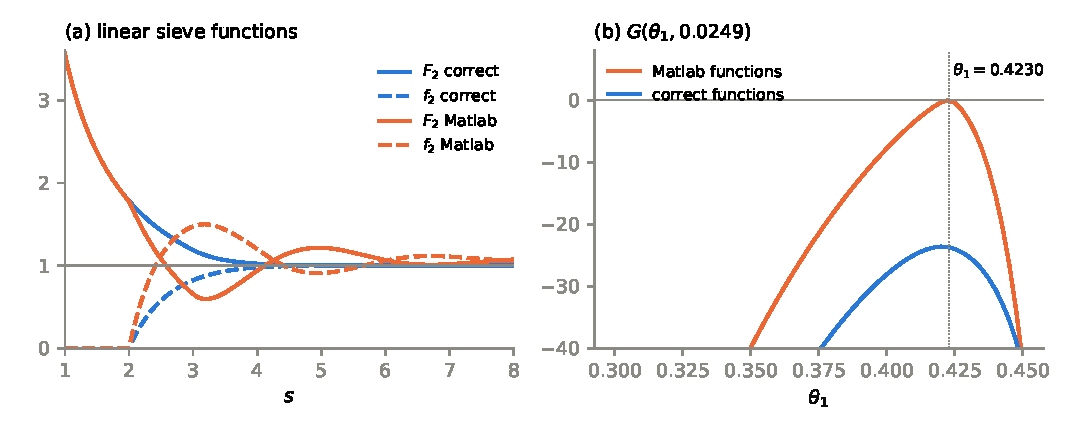
\includegraphics[width=\textwidth]{fig_functions.pdf}
\caption{(a) $F_2$ (solid) and $f_2$ (dashed), correct and as coded. (b) $G(\theta_1,0.0249)$ with the code's
functions and constants, and with the correct functions and the printed constants. The code's curve touches zero at
$\theta_1\approx0.423$, which is where the reported search stopped.}
\label{fig:functions}
\end{figure}

\section{The values at the authors' points}\label{sec:points}

\subsection{The unweighted point}
At $(\theta_1,\theta_2)=(0.4230,0.0249)$ we have $\sigma_1=1.182033$ and $\sigma_2=20.080321$. The constraint in
\eqref{eq:f} is $\theta_1s_1+\theta_2s_2=\frac12$ with $s_1\ge1$ and $s_2\ge2$, so it confines $s_1$ to
$[1,1.0643]$ and $s_2$ to $[2,3.0924]$. On this segment $f_1(s_1)/F_1(s_1)\le0.25$ and $F_2>f_2$, so the bracket
$f_1/F_1+f_2/F_2-1$ is negative throughout. The supremum is $f(\sigma_1,\sigma_2)=-0.40859$, attained near
$(s_1,s_2)=(1.003,3.042)$. With the code's functions the sign of $f_2-F_2$ is reversed on most of the segment, and
the supremum becomes $+1.34662$.

The value of the expression in \eqref{eq:f} at $(s_1,s_2)=(\sigma_1,\sigma_2)$ itself is $f_1(\sigma_1)=0.574$,
since $F_2=f_2=1$ to working accuracy at $s=20$. This point is not admissible, because
$\sigma_1/\sigma_1+\sigma_2/\sigma_2=2$. So no reading of \eqref{eq:f} that evaluates at $(\sigma_1,\sigma_2)$, or
that replaces the supremum by an infimum, is the quantity of Proposition~3.10.

\begin{table}[htbp]
\centering\small
\begin{tabular}{lccccc}
\toprule
functions and constants & $f(\sigma_1,\sigma_2)$ & main & switched & $G(0.4230,0.0249)$\\
\midrule
code: Matlab functions and constants & $1.34662$ & $17.9787$ & $17.9797$ & $-0.0009$\\
printed system \eqref{eq:printed} & $-0.33814$ & $-4.5145$ & $18.2759$ & $-22.790$\\
correct functions, printed constants & $-0.40859$ & $-5.4551$ & $18.2759$ & $-23.731$\\
correct functions, corrected constants & $-0.40859$ & $-5.4551$ & $9.5331$ & $-14.988$\\
\midrule
reported in \cite[\S5]{NX} & & & & $0.001378$\\
\bottomrule
\end{tabular}
\caption{The unweighted criterion at the authors' point. ``Main'' and ``switched'' are the first two terms of
\eqref{eq:H}.}
\label{tab:G}
\end{table}

The code computes $C(\theta_1)$ with the weight $(\beta(1-\beta))^{-1/2}$ instead of $\beta^{-1/2}(1-\beta)^{-1}$
(\texttt{compute\_C\_theta1.m}). This gives $0.170228$ instead of $0.173147$ at $\theta_1=0.4230$; it accounts for
the difference between the switched terms in the first and second rows of Table~\ref{tab:G}. We also replicate
the search in \texttt{find\_theta\_values\_G.m}: $\theta_2$ decreases from $0.04$ in steps of $10^{-4}$, and
$\theta_1$ increases from $0.251$ in steps of $10^{-3}$ until $G>0$. With the code's functions and constants, and a
grid supremum in place of \texttt{fmincon}, the search stops at $\theta_2=0.0248$, $\theta_1=0.422$. This agrees
with the reported $\theta_2=0.0249$, $\theta_1=0.4230$, and $G=0.001378$ is the value of a function that just
crosses zero there (Figure~\ref{fig:functions}(b)). With the correct functions,
$\max_{\theta_1}G(\theta_1,0.0249)<-23$.

\subsection{The weighted point}
At $(\lambda,\theta,\theta_1,\theta_2)=(0.17,0.25,0.449,0.011)$ the constraint in \eqref{eq:f} confines $s_1$ to
$[1,1.0646]$ and $s_2$ to $[2,4.6364]$. For $I$, \texttt{compute\_I.m} calls \texttt{upper\_F\_sigma.m}, which
minimises $F_1F_2$ over the box $s_1\ge1$, $s_2\ge2$ instead of the set in \eqref{eq:F}. For $\alpha>0.029$ this box
does not meet the constraint line, and \texttt{fmincon} then stops at the bound point $(1,2)$, which minimises the
violation of the equality constraint, so that it returns $F_1(1)F_2^{\rm code}(2)=2.68212$. Reproducing this
behaviour gives $I=4.5284$ and $H=1.2625$; the reported value is $1.2690$. Table~\ref{tab:H} lists the values with
$I$ computed from the definition \eqref{eq:F}.

\begin{table}[htbp]
\centering\small
\begin{tabular}{lcccccc}
\toprule
functions and constants & $f$ & $I$ & main & switched & $\lambda\cdot$Richert & $H$\\
\midrule
code, with \texttt{fmincon} at $(1,2)$ & $1.50318$ & $4.5284$ & $44.094$ & $20.249$ & $22.582$ & $1.2625$\\
code functions, $I$ from \eqref{eq:F} & $1.50318$ & $3.0074$ & $44.094$ & $20.249$ & $14.997$ & $8.847$\\
correct functions, printed constants & $0.12546$ & $3.5099$ & $3.680$ & $20.457$ & $17.503$ & $-34.280$\\
correct functions, corrected constants & $0.12546$ & $3.5099$ & $3.680$ & $10.671$ & $17.503$ & $-24.494$\\
\midrule
reported in \cite[\S5]{NX} & & & & & & $1.2690$\\
\bottomrule
\end{tabular}
\caption{The weighted criterion at $(\lambda,\theta,\theta_1,\theta_2)=(0.17,0.25,0.449,0.011)$.}
\label{tab:H}
\end{table}

\section{The switched term}\label{sec:constants}

We go through the proof of \cite[Proposition~4.2]{NX}. Write $L=\log x$. After switching, the sum $T$ over
$x^{\theta_1}<p_1\le x^{1/2}$ counts $p-1=2mp_1p_2$, where every prime factor of $m$ is $\equiv1\ (4)$, and is
bounded by two linear upper-bound sieves: $\lambda_1^+$ of level $D_1$ detects that $2mp_1p_2+1$ is prime, and
$\lambda_2^+$ of level $D_2$ detects that $(2mp_1p_2+3,P(x^{\theta_2}))=1$. The sieve sum is
\begin{equation}\label{eq:sieve-sum}
\Sigma(m)=\sum_{\substack{(d_1,2m)=(d_2,6m)=1\\(d_1,d_2)=1}}\frac{\lambda_1^+(d_1)\lambda_2^+(d_2)}{\varphi(d_1)\varphi(d_2)} .
\end{equation}

\subsection{The joint singular series}
The weights $h(d_1,d_2)=\varphi(d_1)^{-1}\varphi(d_2)^{-1}\mathbf 1_{(d_1,d_2)=1}$ in \eqref{eq:sieve-sum} have
$h^*(p)=h(p,1)+h(1,p)-h(p,p)=2/(p-1)$ for $p\nmid6m$, in the notation of \cite[(3.10)]{NX}. Proposition~3.10 of
\cite{NX}, applied to \eqref{eq:sieve-sum}, gives
\[
\Sigma(m)\le(1+o(1))\,F_2(s_1)F_2(s_2)\,V_1(D_1^{1/s_1})V_2(D_2^{1/s_2})\prod_{p\nmid6m}
\frac{1-\frac2{p-1}}{\bigl(1-\frac1{p-1}\bigr)^2},
\]
where $V_1,V_2$ are the one-dimensional products for $d_1$ and $d_2$, and
$(1-\frac2{p-1})(1-\frac1{p-1})^{-2}=1-(p-2)^{-2}$. In \cite{NX} this factor appears as
$C_1=\prod_{p\nmid6m}(1+(p-2)^{-2})$. The one-dimensional products contribute
$H_1(m)=\frac{2m}{\varphi(2m)}\prod_{p\nmid2m}(1-(p-1)^{-2})$ and the analogous $H_2(m)$, as in \cite{NX}. Since
the factors are less than $1$, a product over $p\nmid2m$ is at least the product over all $p>2$. So
\[
H_1(m)=\frac{2m}{\varphi(2m)}\,c_2\prod_{p\mid m}\Bigl(1-\frac1{(p-1)^2}\Bigr)^{-1}\ \ge\ \frac{2m}{\varphi(2m)}\,c_2,
\]
and the inequality $H_1(m)\le\frac{2m}{\varphi(2m)}c_2$ in \cite{NX} is reversed. The same holds for $H_2$. Keeping
all factors exactly, the per-prime factor for $p>3$ is $k_p=(1-(p-1)^{-2})^2(1-(p-2)^{-2})$ if $p\nmid m$ and $1$ if
$p\mid m$. Hence
\begin{equation}\label{eq:Sigma}
\Sigma(m)\le(32+o(1))\,c_1^{\rm joint}c_2^2\,\frac{m^2}{\varphi(m)^2}\prod_{p\mid m}k_p^{-1}\cdot
\frac{1}{(\log D_1)(\log D_2)}\qquad(D_2=x^{\theta_2}),
\end{equation}
with $c_1^{\rm joint}=\prod_{p>3}(1-(p-2)^{-2})=0.819802$ in place of $c_1=1.202503$. The factor $32$ and the
normalisation are those of \cite{NX}: $8c_1^{\rm joint}c_2^2=\frac92\prod_{p>3}k_p$. The factor
$\prod_{p\mid m}k_p^{-1}$ goes into the sum over $m$.

\subsection{The Wirsing constant}
The sum over $m$ is
\[
S_2(t)=\sum_{m\le t}\frac{b^*(m)\,m}{\varphi(m)^2}=\sum_{m\le t}\frac{g(m)}m,\qquad g(m)=\frac{b^*(m)\,m^2}{\varphi(m)^2},
\]
where $b^*(m)=1$ if every prime factor of $m$ is $\equiv1\ (4)$, and $b^*(m)=0$ otherwise.
Proposition~A.3 of \cite{Martin} (equivalently Wirsing's theorem \cite{Wirsing}) gives
$S_2(t)\sim c_3(\log t)^{1/2}$ with
\begin{equation}\label{eq:c3}
c_3=\frac{1}{\Gamma(3/2)}\prod_{p}\Bigl(1-\frac1p\Bigr)^{1/2}\sum_{k\ge0}\frac{g(p^k)}{p^k}
=\frac{2}{\sqrt\pi}\Bigl(\frac12\Bigr)^{1/2}\prod_{p\equiv1(4)}\Bigl(1-\frac1p\Bigr)^{1/2}
\Bigl(1+\frac{p^2}{(p-1)^3}\Bigr)\prod_{p\equiv3(4)}\Bigl(1-\frac1p\Bigr)^{1/2}.
\end{equation}
The product runs over all primes, and $b^*(2^k)=0$ for $k\ge1$ contributes $(1-\frac12)^{1/2}$. This factor is
missing from \cite[(4.20)]{NX}. The two remaining products diverge separately, since their factors are
$1\pm\frac1{2p}+O(p^{-2})$. They converge together in the order of increasing $p$, because
$\prod_{p\le z}(1-\chi_{-4}(p)/p)\to4/\pi$. In this order the printed expression equals
$\prod_{p\equiv3(4)}(1-p^{-2})^{1/2}\prod_{p\equiv1(4)}(1-\frac1p)(1+\frac{p^2}{(p-1)^3})=1.060689$, and the
truncation at $10^4$ in \texttt{compute\_c3.m} gives $1.061373$. The correct constant is $c_3=1.060689/\sqrt2=0.750020$.

A direct summation over all $m\le10^7$ with $b^*(m)=1$ confirms this. A two-term fit $S_2(t)=c\sqrt{\log t}+d/\sqrt{\log t}$
through $t=10^6$ and $t=10^7$ gives $c=0.7497$ (Table~\ref{tab:c3}). With the weights $\prod_{p\mid m}k_p^{-1}$ of
\eqref{eq:Sigma}, the constant becomes
\[
c_3''=\frac{1}{\sqrt2}\prod_{p\equiv3(4)}(1-p^{-2})^{1/2}\prod_{p\equiv1(4)}\Bigl(1-\frac1p\Bigr)
\Bigl(1+\frac{p^2}{(p-1)^3k_p}\Bigr)=0.811558,
\]
and the same fit gives $0.8112$.

\begin{table}[htbp]
\centering\small
\begin{tabular}{rcccc}
\toprule
$t$ & $S_2(t)$ & $S_2(t)/\sqrt{\log t}$ & $S_2''(t)$ & $S_2''(t)/\sqrt{\log t}$\\
\midrule
$10^4$ & $2.36892$ & $0.78057$ & $2.54818$ & $0.83964$\\
$10^5$ & $2.62724$ & $0.77430$ & $2.82923$ & $0.83383$\\
$10^6$ & $2.86262$ & $0.77016$ & $3.08509$ & $0.83001$\\
$10^7$ & $3.08028$ & $0.76724$ & $3.32151$ & $0.82733$\\
\midrule
fit $c$ & & $0.7497$ & & $0.8112$\\
prediction & & $c_3=0.7500$ & & $c_3''=0.8116$\\
\bottomrule
\end{tabular}
\caption{Direct summation of $S_2(t)$, and of $S_2''(t)$ with the weights $\prod_{p\mid m}k_p^{-1}$. The printed
constant would predict $S_2(t)/\sqrt{\log t}\to1.0607$.}
\label{tab:c3}
\end{table}

\subsection{The levels}
In \cite{NX} the levels satisfy $D_1\le x^{\theta_1}$ and $D_2\le x^{\theta_2}$, and the choice
$D_1=x^{\min(\theta_1,1/2-\theta_2)}$, $D_2=x^{\theta_2}$ gives the factor
$(\theta_2\min(\theta_1,\frac12-\theta_2))^{-1}$. The error terms (4.13)--(4.16) of \cite{NX} use
only $4D_1D_2\le x^{1/2}(\log x)^{-B}$. For the first sieve, take $D_1=x^{1/2-s\theta_2}(\log x)^{-B}$. Since $F_2(s_1)=2\eg/s_1$ on $(0,3]$, any sifting
range $z$ with $D_1^{1/3}\le z\le D_1$ gives $F_2(s_1)V_1(z)=(2+o(1))H_1/\log D_1$, where $s_1=\log D_1/\log z$. In
particular the range $z=x^{\theta_1}$ may be kept whenever $D_1\ge x^{\theta_1}$: then
$1\le s_1=(\frac12-s\theta_2)/\theta_1<2$, because $\theta_1>\frac14$. Otherwise take $z=D_1$.
The second sieve, of level $D_2=x^{s\theta_2}$ with $s\ge1$ and sifting range $x^{\theta_2}$, gives
$F_2(s)V_2(x^{\theta_2})=F_2(s)e^{-\gamma}H_2/(\theta_2L)$. Hence $(\theta_2\min(\theta_1,\frac12-\theta_2))^{-1}$
may be replaced by
\begin{equation}\label{eq:W}
W(\theta_2)=\min_{1\le s<1/(2\theta_2)}\frac{e^{-\gamma}F_2(s)/2}{\theta_2\,(\frac12-s\theta_2)} .
\end{equation}
At $s=1$ this is $(\theta_2(\frac12-\theta_2))^{-1}$. For small $\theta_2$ the minimum lies at $s\approx4.6$, where
$F_2(s)\approx1.005$ instead of $F_2(1)=2\eg$.

\begin{proposition}\label{prop:switch}
Let $\frac14<\theta_1<\frac12$ and $0<\theta_2<\theta_1$. Then
\[
\sum_{\substack{x^{\theta_1}<p_1\le x^{1/2}\\p_1\equiv3(4)}}S(\mathcal A_{p_1},\mathcal Q,p_1)\le
\bigl(2c_1^{\rm joint}c_2^2c_3''\,C(\theta_1)\,W(\theta_2)+o(1)\bigr)\frac{x}{(\log x)^{5/2}},
\]
with $2c_1^{\rm joint}c_2^2c_3''=0.579909$, against $2c_1c_2^2c_3=1.111744$ in \cite[Proposition~4.2]{NX}.
\end{proposition}

\begin{proof}
The proof of \cite[Proposition~4.2]{NX} applies verbatim up to \eqref{eq:sieve-sum}. Bound $\Sigma(m)$ by
\eqref{eq:Sigma}, with $D_1=x^{1/2-s\theta_2}(\log x)^{-B}$ and $D_2=x^{s\theta_2}$, where $1/\log D_2$ is replaced
by $e^{-\gamma}F_2(s)/(2\theta_2\log x)$ as in \eqref{eq:W}, and carry the factor
$\prod_{p\mid m}k_p^{-1}$ into the sum over $m$. The function $g(m)\prod_{p\mid m}k_p^{-1}$ satisfies the hypotheses
of \cite[Proposition~A.3]{Martin} with $\kappa=\frac12$, because $k_p=1+O(p^{-2})$. The remaining steps,
(4.21)--(4.23) of \cite{NX}, are unchanged, with $c_3''$ in place of $c_3$.
\end{proof}

Items (i) and (ii) multiply the switched term by $0.5216$. The error in $H_1$ alone would increase it, but it is
outweighed by the other two.

\section{What the method gives}\label{sec:restore}

We consider three versions of the switched term: R0 uses Proposition~4.2 as printed; R1 uses corrected constants,
$0.579909$ instead of $1.111744$; R2 is Proposition~\ref{prop:switch}, which adds the free levels \eqref{eq:W}. In
each case we use the correct functions in \eqref{eq:f} and \eqref{eq:F}. For the unweighted criterion we find the
largest $\theta_2$ such that $G(\theta_1,\theta_2)>0$ for some $\theta_1$. For the weighted criterion we minimise
$1/\lambda+1/\theta$ subject to $H\ge0$. Since $H$ is linear in $\lambda$, we set
$\lambda=(\text{main}-\text{switched})/\text{Richert}$, optimise over $\theta$, and scan $\theta_1$ (step $0.0025$)
and $\theta_2\in[0.0004,0.015]$. The integral $I$ is computed from \eqref{eq:F} on a grid of $161$ nodes in
$\log\alpha$; an independent $160$-point Gauss--Legendre evaluation agrees to $2\cdot10^{-4}$ at every optimum.

\begin{table}[htbp]
\centering\small
\begin{tabular}{lccccccc}
\toprule
& \multicolumn{2}{c}{unweighted} & \multicolumn{5}{c}{weighted}\\
\cmidrule(lr){2-3}\cmidrule(lr){4-8}
& $\theta_2^*$ & $\omega\le$ & $(\theta_1,\theta_2)$ & $\theta$ & $\lambda$ & $1/\lambda+1/\theta$ & $\omega\le$\\
\midrule
R0 & $0.002917$ & $342$ & $(0.4850,0.0006)$ & $0.0825$ & $0.02124$ & $59.20$ & $59$\\
R1 & $0.005627$ & $177$ & $(0.4725,0.0012)$ & $0.1101$ & $0.03216$ & $40.17$ & $40$\\
R2 & $0.020412$ & $48$ & $(0.3975,0.0060)$ & $0.1949$ & $0.08130$ & $17.43$ & $17$\\
\midrule
\cite{NX} & $0.0249$ & $40$ & $(0.449,0.011)$ & $0.25$ & $0.17$ & $9.88$ & $9$\\
\bottomrule
\end{tabular}
\caption{The method of \cite{NX} with the correct sieve functions. ``$\omega\le$'' is
$\lfloor1/\theta_2^*\rfloor$ (unweighted) and $\lceil1/\lambda+1/\theta\rceil-1$ (weighted). Elements $p+2$ that
are not squarefree number $O(x^{1-\theta_2})$, so the same bounds hold for $\Omega(p+2)$.}
\label{tab:restore}
\end{table}

\begin{figure}[htbp]
\centering
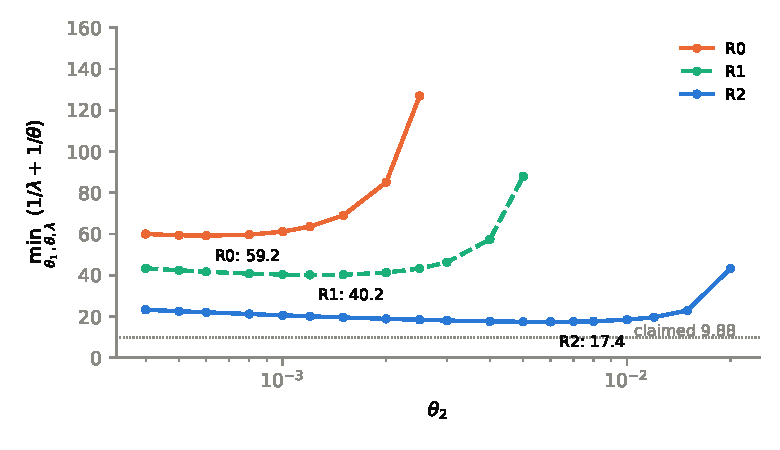
\includegraphics[width=0.72\textwidth]{fig_restore.pdf}
\caption{$\min_{\theta_1,\theta,\lambda}(1/\lambda+1/\theta)$ subject to $H\ge0$, as a function of $\theta_2$, for
R0, R1 and R2.}
\label{fig:restore}
\end{figure}

\begin{proof}[Proof of Theorem~\ref{thm:B}]
Propositions~4.1 and~4.3 of \cite{NX} and Proposition~\ref{prop:switch} give the criterion \eqref{eq:H} with the
switched term of R2. At the R2 point of Table~\ref{tab:restore} the three terms are $32.698$, $15.797$ and
$16.901$, so $H=0$ at $\lambda=0.08130$, and $H>0$ for $\lambda=0.0812$, where $1/\lambda+1/\theta=17.45<18$. The
argument of \cite[\S2]{NX} then gives $\omega(p+2)\le17$ for $\gg x(\log x)^{-5/2}$ primes, and squarefreeness gives
$\Omega(p+2)\le17$. The R0 and unweighted values are obtained in the same way.
\end{proof}

\begin{remark}\label{rem:structure}
The main term needs $f(\sigma_1,\sigma_2)>0$. At $\theta_1$ near $\frac12$ we have $\sigma_1=1+\delta+O(\delta^2)$
with $\delta=1-2\theta_1$, and $f_1(\sigma_1)/F_1(\sigma_1)\sim\sqrt\delta$, while $C(\theta_1)\sim\frac83\delta^{3/2}$.
So the main term beats the switched term only as $\delta\to0$. The constraint $\theta_1+2\theta_2\le\frac12$ then
forces $\theta_2\le\delta/4$, and the Richert integral grows like $\log(\theta/\theta_2)$. This is why R0 and R1
need very small $\theta_2$. In R2 the switched term is small enough that $\theta_1=0.3975$ is admissible.
\end{remark}

\begin{remark}\label{rem:buchstab}
Lemma~4.3 of \cite{ChenXIII} and Section~5 of \cite{ChenXIV} replace the rectangle bounds \eqref{eq:f} and
\eqref{eq:F} on the inert primes by the fixed point of Buchstab's recursion. This leaves the switched term
unchanged and improves the main and Richert terms. With the switched term of R0 it lowers the trapezoid value at
$\theta_2\ge0.002$ from $84.85$ to $56.86$ \cite[\S5]{ChenXIV}. The supplementary script
\texttt{code/part14\_fixed\_point.py} combines that engine with R0--R2. Its rectangle values ($n=400$) reproduce
the table above independently: $17.425$, $40.130$ and $59.158$. With the fixed point and the one-sided (certified)
quadrature at $n=1600$ it gives $1/\lambda+1/\theta=15.947$ for R2 at $(\theta_1,\theta_2)=(0.3991,0.008)$, hence
$\Omega(p+2)\le15$; $38.06$ for R1 at $(0.4725,0.002)$, hence $\Omega(p+2)\le38$; and $58.68$ for R0 at
$(0.4859,0.0006)$, hence $\Omega(p+2)\le58$. The trapezoid values, which are not certified, are $15.72$, $35.79$
and $53.24$. For R2 a finer grid widens the margin below $16$: at $n=3200$ the one-sided value is $15.831$ at
$\theta_2=0.008$ and $15.809$ at $(\theta_1,\theta_2)=(0.3984,0.009)$, against trapezoid values $15.72$ and $15.69$
(\texttt{data/part14\_margin.txt}, computed with \texttt{code/nath\_xie\_margin.py} of \cite{ChenXIV}).
\end{remark}

\section{Further remarks on the text}\label{sec:minor}
\begin{enumerate}
\item In \cite[Lemma~3.6]{NX}, the differential equation for $F_i$ should hold for $s_i>\beta_i+1$, not for
$s_i>\beta_i-1$.
\item In \cite[\S5]{NX}, the printed equation \eqref{eq:printed} for $f_2$ is stated for $s>2$, where it contradicts
the printed initial segment of $f_2$ on $[2,4]$. The correct equation \eqref{eq:lin} is satisfied by that segment
on $(2,4]$.
\item The box $s_1\ge1$, $s_2\ge2$ in \texttt{upper\_F\_sigma.m} differs from \eqref{eq:F}. For an infimum a smaller
set is only conservative, but at most of the range of $I$ the set is empty (Section~\ref{sec:points}).
\item Both optimisation files start \texttt{fmincon} at $(1.5,2.5)$, which does not satisfy the equality
constraint. At the points we tested, the objective of \eqref{eq:f} has a single local maximum on the segment, so
the lower bound itself is unaffected.
\end{enumerate}

\section*{Data and code}
\begin{itemize}
\item \texttt{code/verify\_nath\_xie.py}: pure standard library; all numbers in Sections~\ref{sec:functions}--\ref{sec:restore}
($\approx$15\,s); output \texttt{data/verify\_nath\_xie.txt}. Option \texttt{--quick}: coarser grids.
\item \texttt{code/make\_figures.py}: Figures~\ref{fig:functions} and~\ref{fig:restore} (matplotlib).
\item \texttt{code/part14\_fixed\_point.py}: Remark~\ref{rem:buchstab} (numpy; uses the engine of \cite{ChenXIV}); output
\texttt{data/part14\_fixed\_point.txt}. The file \texttt{data/part14\_margin.txt} is a copy of the output of
\texttt{code/nath\_xie\_margin.py} in the repository of \cite{ChenXIV}.
\end{itemize}
The Matlab files cited are those in the folder \texttt{Computation\_files} of the arXiv source of \cite{NX} (version~3).

\begin{thebibliography}{99}
\bibitem{ChenXIII} R. Chen, Sums of two squares and Heegner norms with few prime factors, XIII: half-dimensional
vector sieves, class-group covering, and explicit small $r$ for arbitrary class pairs $(C',C)$, preprint (2026),
doi:10.5281/zenodo.24125302.
\bibitem{ChenXIV} R. Chen, Sums of two squares and Heegner norms with few prime factors, XIV: the Buchstab fixed
point of a vector sieve as an obstacle problem, causal computation, and variable dispersion levels, preprint (2026),
doi:10.5281/zenodo.24231797.
\bibitem{FI} J. Friedlander and H. Iwaniec, \emph{Opera de cribro}, Amer. Math. Soc. Colloq. Publ. 57, Amer. Math.
Soc., Providence, RI, 2010.
\bibitem{HBL} D. R. Heath-Brown and X. Li, Almost prime triples and Chen's theorem, J. Number Theory 169 (2016),
265--294.
\bibitem{Iw72} H. Iwaniec, Primes of the type $\varphi(x,y)+A$ where $\varphi$ is a quadratic form, Acta Arith. 21
(1972), 203--234.
\bibitem{Martin} G. Martin, An asymptotic formula for the number of smooth values of a polynomial, J. Number Theory
93 (2002), 108--182.
\bibitem{NX} K. Nath and L. Xie, Almost primes and primes that are sums of two squares plus 1, Acta Arith. 223
(2026), no.~1, 51--82, doi:10.4064/aa250227-19-11; arXiv:2501.16723v3 (17 August 2026).
\bibitem{Wirsing} E. Wirsing, Das asymptotische Verhalten von Summen \"uber multiplikative Funktionen, Math. Ann.
143 (1961), 75--102.
\end{thebibliography}
\end{document}
